\documentclass[journal,12pt,twocolumn]{IEEEtran}

\usepackage{setspace}
\usepackage{gensymb}

\singlespacing
% \documentclass{article}
% \usepackage[demo]{graphicx}               
\usepackage[cmex10]{amsmath}

\usepackage{amsthm}
\usepackage{enumerate}
\usepackage{mathrsfs}
\usepackage{txfonts}
\usepackage{stfloats}
\usepackage{bm}
\usepackage{cite}
\usepackage{cases}
\usepackage{subfig}
 
\usepackage{longtable}
\usepackage{multirow}
% \ref{fig:x cubed graph}
\usepackage{enumitem}
\usepackage{mathtools}
\usepackage{steinmetz}
\usepackage{tikz}
\usepackage{circuitikz}
\usepackage{verbatim}
\usepackage{tfrupee}
\usepackage[breaklinks=true]{hyperref}
\usepackage{graphicx}
\usepackage{tkz-euclide}
\usepackage{amsmath}

\usetikzlibrary{calc,math}
\usepackage{listings}
    \usepackage{color}                                            %%
    \usepackage{array}                                            %%
    \usepackage{longtable}                                        %%
    \usepackage{calc}                                             %%
    \usepackage{multirow}                                         %%
    \usepackage{hhline}                                           %%
    \usepackage{ifthen}                                           %%
    \usepackage{lscape}     
\usepackage{multicol}
\usepackage{chngcntr}

\DeclareMathOperator*{\Res}{Res}

\renewcommand\thesection{\arabic{section}}
\renewcommand\thesubsection{\thesection.\arabic{subsection}}
\renewcommand\thesubsubsection{\thesubsection.\arabic{subsubsection}}

\renewcommand\thesectiondis{\arabic{section}}
\renewcommand\thesubsectiondis{\thesectiondis.\arabic{subsection}}
\renewcommand\thesubsubsectiondis{\thesubsectiondis.\arabic{subsubsection}}



\def\inputGnumericTable{}                                 %%

\lstset{
%language=C,
frame=single, 
breaklines=true,
columns=fullflexible
}
\begin{document}


\newtheorem{theorem}{Theorem}[section]
\newtheorem{problem}{Problem}
\newtheorem{proposition}{Proposition}[section]
\newtheorem{lemma}{Lemma}[section]
\newtheorem{corollary}[theorem]{Corollary}
\newtheorem{example}{Example}[section]
\newtheorem{definition}[problem]{Definition}

\newcommand{\BEQA}{\begin{eqnarray}}
\newcommand{\EEQA}{\end{eqnarray}}
\newcommand{\define}{\stackrel{\triangle}{=}}
\bibliographystyle{IEEEtran}
\providecommand{\mbf}{\mathbf}
\providecommand{\pr}[1]{\ensuremath{\Pr\left(#1\right)}}
\providecommand{\qfunc}[1]{\ensuremath{Q\left(#1\right)}}
\providecommand{\sbrak}[1]{\ensuremath{{}\left[#1\right]}}
\providecommand{\lsbrak}[1]{\ensuremath{{}\left[#1\right.}}
\providecommand{\rsbrak}[1]{\ensuremath{{}\left.#1\right]}}
\providecommand{\brak}[1]{\ensuremath{\left(#1\right)}}
\providecommand{\lbrak}[1]{\ensuremath{\left(#1\right.}}
\providecommand{\rbrak}[1]{\ensuremath{\left.#1\right)}}
\providecommand{\cbrak}[1]{\ensuremath{\left\{#1\right\}}}
\providecommand{\lcbrak}[1]{\ensuremath{\left\{#1\right.}}
\providecommand{\rcbrak}[1]{\ensuremath{\left.#1\right\}}}
\theoremstyle{remark}
\newtheorem{rem}{Remark}
\newcommand{\sgn}{\mathop{\mathrm{sgn}}}
\providecommand{\abs}[1]{\l\vert#1\r\vert}
\providecommand{\res}[1]{\Res\displaylimits_{#1}} 
\providecommand{\norm}[1]{\lVert#1\rVert}
%\providecommand{\norm}[1]{\lVert#1\rVert}
\providecommand{\mtx}[1]{\mathbf{#1}}
\providecommand{\mean}[1]{E\l[ #1 \r]}
\providecommand{\fourier}{\overset{\mathcal{F}}{ \rightleftharpoons}}
%\providecommand{\hilbert}{\overset{\mathcal{H}}{ \rightleftharpoons}}
\providecommand{\system}{\overset{\mathcal{H}}{ \longleftrightarrow}}
 %\newcommand{\solution}[2]{\textbf{Solution:}{#1}}
\newcommand{\solution}{\noindent \textbf{Solution: }}
\newcommand{\cosec}{\,\text{cosec}\,}
\providecommand{\dec}[2]{\ensuremath{\overset{#1}{\underset{#2}{\gtrless}}}}
\newcommand{\myvec}[1]{\ensuremath{\begin{pmatrix}#1\end{pmatrix}}}
\newcommand{\mydet}[1]{\ensuremath{\begin{vmatrix}#1\end{vmatrix}}}
\numberwithin{equation}
\makeatletter
\addtoreset{}{}
\makeatother
\let\StandardTheFigure\thefigure
\let\vec\mathbf
\renewcommand{\thefigure}{\theproblem}
\def\putbox#1#2#3{\makebox[0in][l]{\makebox[#1][l]{}\raisebox{\baselineskip}[0in][0in]{\raisebox{#2}[0in][0in]{#3}}}}
     \def\rightbox#1{\makebox[0in][r]{#1}}
     \def\centbox#1{\makebox[0in]{#1}}
     \def\topbox#1{\raisebox{-\baselineskip}[0in][0in]{#1}}
     \def\midbox#1{\raisebox{-0.5\baselineskip}[0in][0in]{#1}}
\vspace{3cm}
\title{Assignment 2}
\author{T.Guru Balaji}
\maketitle
\newpage
\bigskip
\renewcommand{\thefigure}{\theenumi}
\renewcommand{\thetable}{\theenumi}
Download all python codes from 
\begin{lstlisting}
https://github.com/TGURUBALAJI/INTERNSHIP-IITH/Assignment2/code
\end{lstlisting}
%
and latex-tikz codes from 
%
\begin{lstlisting}
https://github.com/TGURUBALAJI/INTERNSHIP-IITH/Assignment2/gbalaji.tex
\end{lstlisting}
\vskip 1cm
\textbf{2.106 }Find the values of $k$ for which the line
\begin{align}
\myvec{k-3 \hspace{4mm}-\myvec{4-k^2}}\vec{x}+k^2-7k+6=0
\end{align}
is\\
a) Parallel to the x-axis\\
b) Parallel to the y-axis\\
c) Passing through the origin\\
%
\vskip 0.5cm
\textbf{Solution} Given equation of the line, 
\begin{align}
\myvec{k-3 \hspace{4mm}-\myvec{4-k^2}}\vec{x}+k^2-7k+6=0\label{eq:1}
\end{align}
\begin{center}
 \begin{sloppypar}of a general line equation\hspace{4mm} ${\vec{nx = }\hspace{2mm}c}$\newline
here ${\vec{n}=\myvec{k-3 \hspace{3.5mm}-\{4-k^2\}}}$\newline
and\hspace{4mm} ${c = -k^2+7k-6}$\end{sloppypar}\end{center}
\begin{enumerate}[label=\emph{\alph*)}]
\item Parallel to x-axis\\
$\vec{n}=\myvec{0 & 1}$ if the line is parallel to x-axis\\
Equation of x-axis is $\myvec{1 & 0}\vec{x}=0$\
\begin{align}
  \myvec{1 & 0}\myvec{k-3\\-\{4-k^2\}} =0
\end{align}
\begin{align}
   k-3=0
\end{align}
\begin{align}
    k=3
\end{align}
Substituting $k=3$ in \eqref{eq:1}\\
Equation of line is,
\begin{align}
     \myvec{0 & 5}\vec{x}=6
\end{align}
 
\item Parallel to y-axis\\
$\vec{n}=\myvec{1 & 0}$ if the line is parallel to y-axis\\
Equation of y-axis is $\myvec{0 & 1}\vec{x}=0$\\
\begin{align}
  \myvec{0 & 1}\myvec{k-3\\-(4-k^2)} =0
\end{align}
\begin{align}
   4-k^2=0
\end{align}
\begin{align}
    k=\pm2
\end{align}
Substituting $k=2$ in \eqref{eq:1}.
Equation of line is,
\begin{align}
     \myvec{-1 & 0}\vec{x}= 4
\end{align}
Substituting $k=-2$ in \eqref{eq:1}.
Equation of line is,
\begin{align}
  \myvec{-5 & 0}\vec{x}=-24
\end{align}
\item Passing through origin\\
${c = 0}$ \hspace{4mm}if the line passes through origin\\
Equation of line when passing through origin is 
\begin{align}
\vec{n}^\top\vec{x}=0
\end{align}
Hence
% \begin{align}
%     -k^2+7k-6=0  (k-1)(k-6)=0 \implies k=1, k=6
% \end{align}
\begin{equation} \label{eq1}
\begin{split}
-k^2+7k-6 & = 0 \\
 & = -k^2+k+6k-6\\
 & = (k-1)(k-6)\\
 \implies k=1, k=6
\end{split}
\end{equation}
Substituting $k=1$ in \eqref{eq:1}.
The equation of line is,
\begin{align}
\myvec{-2&-3}\vec{x} = 0
\end{align}
Substituting $k=6$ in \eqref{eq:1}.
The equation of line is,
\begin{align}
  \myvec{3 & 32}\vec{x} = 0
\end{align}
\end{enumerate}
\begin{figure}[!h]
         \centering
         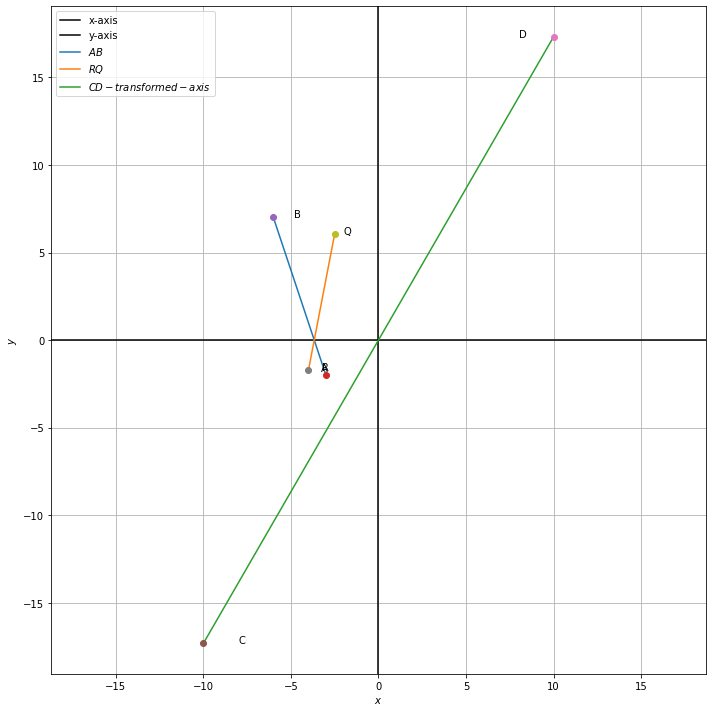
\includegraphics[width=\columnwidth]{image.png}
         \caption{Plot of line equations}
         \label{fig:x cubed graph}
\end{figure}
\end{document}
